	\documentclass[11pt]{article}
%Gummi|063|=)
\title{\textbf{Image Processing}}
\author{}
\date{}
\usepackage{amsmath}
\usepackage{graphicx}
\usepackage{listings}
\begin{document}

\maketitle

\section{Abstract}
Our group chose to use our existing knowledge of linear algebra and differential equations and apply it to the field of image processing. Our system is a python module that can apply a linear transformations to an image of any size. It is capable of rotating, scaling, and changing the color balance of images. In addition, we looked into convolution based operations like Sobel edge detection, Laplacian edge detection and Gaussian blur.

\section{Functionality}
\subsection{Translation Matrix}
For our first feature we implemented various transforms. To do this we first have to express our large image matrix in a way in which we can apply a transformation matrix. When we first import an image we import it as n by m by 3(r,g,b) matrix where n and m are the size of the image. This matrix needs to be converted to a 6 by n*m matrix
$$\begin{pmatrix}
	x & 0 & ...\\
	y & 0 & ...\\
	1 & 1 & ...\\
	r &  255 & ...\\
	g & 255 & ...\\
	b & 255 & ...\\
\end{pmatrix}$$
 With this matrix, One can simply apply a transformation matrix with a 3x3 identity in the lower corner right hand corner. For example a rotation matrix is:
 $\begin{pmatrix} 
	cos(\theta) & -sin(\theta) & 0 & 0 & 0 & 0\\
	sin(\theta) & cos(\theta) & 0 & 0 & 0 & 0\\
	0 & 0 & 1 & 0 & 0 & 0\\
	0 & 0 & 0 & 1 & 0 & 0\\
	0 & 0 & 0 & 0 & 1 & 0\\
	0 & 0 & 0 & 0 & 0 & 1\\
\end{pmatrix}$

A demo translation matrix is:
  $\begin{pmatrix}
	1 & 0 & dx & 0 & 0 & 0\\
	0 & 1 & dy & 0 & 0 & 0\\
	0 & 0 & 1 & 0 & 0 & 0\\
	0 & 0 & 0 & 1 & 0 & 0\\
	0 & 0 & 0 & 0 & 1 & 0\\
	0 & 0 & 0 & 0 & 0 & 1\\
\end{pmatrix}$
where dx and dy are your translation.

Although these transformations work great in this format this is not the format needed to export the image. When doing these transformations, the xy coordinates of each pixel might be mapped to a non integer value. To recreate the image, we must first sample this list and interpolate between points that are close to each pixel in the new image.


\subsection{Flipping}
Another way to do manipulation of an image is via a rotated identity matrix. 

$A = \begin{pmatrix}
	0 & 0 & 0 & 1\\
	0 & 0 & 1 & 0\\
	0 & 1 & 0 & 0\\
	1 & 0 & 0 & 0\\
\end{pmatrix}$

One can then use this to flip an image both vertically and horizontally.
If matrix $P$ is ones image, one can flip horizontally with:
$A P$ and vertically with $P A$. 

\subsection{Convolution}
Convolution can be thought of as blending two functions together. For our project we mainly focused on discrete convolution. Convolution is simply a linear operator and we can analyse it that way. 

Given vector
$ A = \begin{pmatrix}
	0 & 0 & 0 & 1 & 2 & 3 & 4 & 4 & 4\\
\end{pmatrix}$

and Kernel $K = \begin{pmatrix}
	1 & 1 & 1 \\
\end{pmatrix}$

To convolve $A$ and $K$, $S = A*K$ one needs to place the kernel over the image at each point of A. To solve for the first index of the solution vector, $S_0 = A_{-1}K_{0}+A_{0}K_{1}+A_{1}K_{2}$ To solve for $S_N = A{N-1}K_{0}+A{N}K_{1}+A{N+1}K_{2}$. The one thing that is not defined is what to do with the negative indexes. A simple solution one can do, a simplifying function that makes math easier, is to assume that $A_{-1} = A_{N-1}$. With this assumption made, the solution to this convolution is simply 
$ S = \begin{pmatrix}
	4 & 0 & 1 & 3 & 6 & 10 & 11 & 12 & 8\\
\end{pmatrix}$

Quantitatively, this kernel adds the two adjacent values to itself. Because convolution is a linear transformation, one can write a matrix for this. Because we made the assumption that the indices loop, we can write our matrix as a circulant matrix. 

For this kernel, a sample convolution matrix would look like, assuming size 5 vector. 

$\begin{pmatrix}
	1 & 1 & 0 & 0 & 1\\
	1 & 1 & 1 & 0 & 0\\
	0 & 1 & 1 & 1 & 0\\
	0 & 0 & 1 & 1 & 1 \\
	1 & 0 & 0 & 1 & 1\\
\end{pmatrix}$

Each row is just a rotated version of the row above it. This pattern holds for any size matrix.

A more general form of this is:
$$\begin{matrix}
	c_0 & c_{n-1} & \cdots & c_2 & c_1\\
	c_1 & c_0 & c_{n-1} &  & c_2\\
	\vdots & c_1 & c_0 & \ddots & \vdots\\
	c_{n-2} &   & \ddots & \ddots & c_{n-1}\\
	c_{n-1} & c_{n-2} & \cdots & c_1 & c_0\\
\end{matrix}$$

where c is your convolution kernel. 

Because this matrix follows a specific form, its eigen values and vectors are defined and in a specific form.

$$v_j = (1, w_j, w_j^2, w_j^3, ..., w_j^{n-1})$$
$$\lambda_j =c_0+c_{n-1}w_j	+c_{n-2}w_j^2+...+c_{1}w_j{n-1}2$$

Where $w$ are the roots of unity,
$$w_j = e^{\dfrac{2\pi i j}{n}}$$
and where n is the amount of discrete points one has.
 
 To find the eigen values of the above kernel for a discrete vector of size n one would just substitute in values of c. $c_1 = 1, c_0 = 1, c_{n-1}=1$
 $$\lambda_j =1+c_{n-1}e^{\dfrac{2\pi i j}{n}}+c_{1}e^{(n-1) \dfrac{2\pi i j}{n}}$$
 because we are working in this cyclic system, one can rewrite $n-1$ as $1$. 
 $$\lambda_j = 1+w_j+w_j^{-1}$$
 $$\lambda_j =1+e^{\dfrac{2\pi i j}{n}}+e^{\dfrac{-2\pi i j}{n}}$$
and fianlly via Euler formula, 
$$\lambda_j = 2 \cos(\dfrac{2\pi j}{n})+1$$
To do further analysis on this, one can see that the dominant eigen value occurs when $\cos(\dfrac{2 \pi j}{n})$ is at a maximum. when j is small. The maximum eigen value, $\lambda_0 = 3$. 
One can now look at the dominant eigen vector,
$$v_0 = (1,1,1....)$$. 

looking at another eigen vector, say $n/2$ would yeild: 
$$v_{n/2} = (1, -1, 1, -1, ....$$ This corresponds to the highest frequency possible. When looking at the eigen value for this case, $\lambda_{n/2}=-1$. This value is low in magnitude, thus not many high frequency features come through after the filter.

It is interesting to note that the eigen vectors of a discrete convolution do not change with respect to kernel that one is convolving against. They will always be sinusoidal waves increasing in frequency. 

When thinking about this quantitatively one can see that this eigen value corresponds to a low frequency. This makes intuitive sence when one looks at the above kernel. It adds the two adjacent places to itself. This bluing of sorts is expressed here. Low frequencies have a high magnitude eigen values, thus they are preserved. High frequencies have lower magnitude eigen values, thus removing them.
Another interesting note about this is that the maximum eigen value is equal to 3. This is equal to the total amplification of the image. If one was to add the kernel up, they would also get three. 

Another interesting thing to think about is the null space of this filter. When thinking about it in terms of bluring, one can see that there would be no null space. This is also confirmed by taking the determinate, which is non zero. 

One can extend this 1d analagy to two d. One can simply just make a long list of every pixel. Although this would work, it is quite ugly to write kernels for. 

This is when 2D convolution comes in. It can be thought of as super imposing the flipped kernel on top of the image and adding together each entry of the kernel multiplied by the original much like how 2d works, except in 3d.
Figure 1 sums up the process.

\begin{figure}[Htp]
%\centering
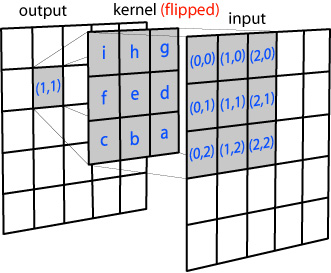
\includegraphics[width=3in]{conv2d_matrix.jpg}
\caption{Convolution in 2D.}
\label{}
\end{figure}

\subsection{Gaussian Blur}
A Gaussian function is simply just a normal distribution. This function is defined by:

$$
G(x,y) = \dfrac{1}{2\pi \sigma^2}e^{-\dfrac{x^2+y^2}{2 \sigma^2}}$$

Where sigma is the standard deviation for the curve, which in this application is how much blur to apply.

To apply this function to the image we use convolution. Because we are using discrete data, we use a discrete convolution. To do this convolution we need to first choose a kernel size for our Gaussian function. The Gaussian function never goes to zero, it only crouches zero. A kernel that is the size of the image would be ideal, but it is unneeded because values further away from the 0,0 point are very close to zero. For our tests, we used kernel sizes of (5,5) to (21,21), assume the rest are zeros. These gave us good results while still being fairly efficient to compute. 

To analyse this filter we will once again reduce it to one dimension. The formula for the Gaussian function in 1d is:  
$$ G(x) = \dfrac{1}{\sqrt{2\pi \sigma^2}}e^{\dfrac{-x^2}{2\sigma^2}} $$
One can convert this to a discrete kernel by simply plugging in values into kernel $c$.
Once again, like above, this convolution creates a circulant matrix. With this matrix known, one can again find the formula for the eigen values using:
$$\lambda_j = c_0+c_{n-1}w_j+c_{n-2}w_j^2 + ... + c_1w_j^{n-1}$$

Because $G(x)$ is always positive, this expression simplifies to be $$\lambda_j = c_0+(c_{1}+c_{n-1})\cos(\dfrac{2\pi j}{n})(c_{2}+c_{n-2})\cos(\dfrac{4\pi j}{n}) ...$$ for symmetric matrix. Once again, the maximum eigen value occurs when the $\cos$ term is at a maximum, thus j=0. Again this matches with the previous example, because this function also applies a form of blur.   

\subsection{Laplacian edge detection}
The next filter we chose to implement was a Laplacian operator, or a second derivative in 1d. To do this, one first has to think about discrete derivatives.
\begin{figure}[htp]
%\centering
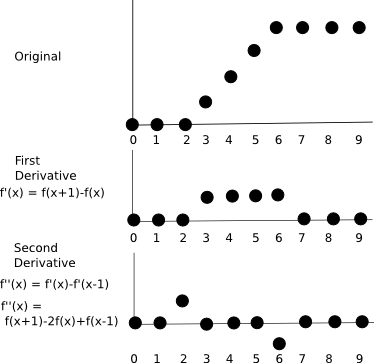
\includegraphics[width=3in]{discreteLaplacian.png}
\label{}
\end{figure}
The rational for choosing first a point ahead and then a point behind was to try to limit the amount of nearby points needed to sample, but not offset the derivatives. This is why I did one from each. When looking at the final expression for f''(x), one can see that the convolution kernel needs to be $(1,-2,1)$.

We can analyse this kernel the same way that we analysed the above. Jumping right to the the generalized solution for symmetric kernels,$$\lambda_j = c_0+(c_{1}+c_{n-1})\cos(\dfrac{2\pi j}{n})(c_{2}+c_{n-2})\cos(\dfrac{4\pi j}{n}) ...$$ 
$$ \lambda_j = -2 + 2\cos(\dfrac{2\pi j}{n}) $$. The dominant eigen value for this will be negative, with a value of j equal to $n/2$. When finding the eigen vector at this point, one gets from above $v_{n/2} = (1,-1,1,-1, ...)$. This means that high frequency changes are preserved. 

When thinking about what this filter is actually doing this makes sense. This is an edge detection filter. It looks for very rapid changes and calls them edges and looses the rest.

Another interesting property of this filter is that if one was to add all of the values in the kernel together they would get zero. This correlates to having a nullspace. A image that has no changes, low low frequency, a flat color, one would get only black, or zero.

Another interesting fact about this filter is that it is sign independent. The filter is comparing its position to its neighbours, thus sign does not effect its ability to detect edges.  
 
To extend this filter into two dimensions is complicated and can be done with analysis like we did above except in 2d. Ones filters will change depending on how one defines the discrete differentiation.

To do this, we used the following discrete kernel:
$\begin{pmatrix}
	-1 & -1 & -1\\
	-1 & 8 & -1\\
	-1 & -1 & -1\\
\end{pmatrix}$


\subsection{Sobel Edge Detection}
Another filter we analysed was the Sobel operator. The Sobel operator is technically a discrete differential operator in 2d. Basically we are calculating the gradient for the function. This gradient can be expressed as two kernels. One for the derivative in the x direction and one for the derivative in the y direction.

Kernel in the X direction:
$K_x = \begin{pmatrix}
	-1 & 0 & 1\\
	-2 & 0 & 2\\
	-1 & 0 & 1\\
\end{pmatrix}$

Kernel in the Y direction:
$K_y = \begin{pmatrix}
	-1 & -2 & -1\\
	0 & 0 & 0\\
	1 & 2 & 1\\
\end{pmatrix}$

These two filters are developed by a multiplication of two vectors, a 1d sobel operator, and a 1d smoothing average of sorts. 


$$\begin{pmatrix}
	1\\
	2\\
	1\\
\end{pmatrix}\begin{pmatrix}
	-1 & 0 & 1\\
\end{pmatrix} = \begin{pmatrix}
	-1 & 0 & 1\\
	-2 & 0 & 2\\
	-1 & 0 & 1\\
\end{pmatrix}$$
$$\begin{pmatrix}
	-1\\
	0\\
	1\\
\end{pmatrix}\begin{pmatrix}
	1 & 2 & 1\\
\end{pmatrix} =\begin{pmatrix}
	-1 & -2 & -1\\
	0 & 0 & 0\\
	1 & 2 & 1\\
\end{pmatrix}$$

Because these kernels are separate, we can analyse them in parts. We have analyzed many filters like the (1,2,1) filter earlier, it is a burring of sorts. It will bring through low frequencies and drop high frequencies. 

The interesting filter here is the sobel operator. First I will find there eigen values.

$$\lambda_j = 0 + e^{\dfrac{2\pi i j}{n}}-e^{\dfrac{-2\pi i j}{n}}$$
This simplifies to
$$\lambda_j = 2i\sin(\dfrac{2 \pi j}{n})$$
As one can see these eigen values are entirely imaginary. The magnitude is at a maximum at $j=n/4$ and at a minimum at $j=0$ and $j=n/2$. This makes sense in two respects. The first is that all of the values are imaginary. This means that there is a phase shift. Because this is an approximation of a derivative also has a phase shift of 90 degrees.

The other reason this makes sense is when the value is at its maximum. The eigen value for this is $v_{n/4} = (1,1i,-1,-1i,1, 1i, ...)$ . This oscillates from real to imaginary every value. To give a real example of the effect would be on the following dataset. 
$$d = (1,0,-1,0,1,0,-1,0)$$
Applying this kernel would yeild:
$$d*k = (0,-2,0,2,0,-2,0,2)$$. 
This shows the phase shift and the amplification. 

In 2d, one can convolute the image, A, against the two kernels. $x = A*K_x$ and $y=A*K_y$. 

One can then take distance $\sqrt(x^2+y^2)$ between these two values, to get the edges. 


\subsection{Blur + edge detection}
Another interesting thing to note about edge detection is that one can tune how small the edges should be. This can be done by applying a Gaussian blur before this filter. One softens all of the high frequencies by blurring and then picks out the remaining ones. 
Because convolution is commutative and associative, it does not matter which order one takes the convolutions.

\subsection{Color Transformation}
Our images are made up of three channels, red, green, and blue. One can manipulate these channels to change how the colors are represented. For example, to output a gray scale, one can simply average all three channels and output 3 of that average for all red, green and blue channels.

To increase or decrease the brightness, one can multiply by a some constant. If this constant is greater than one, the image becomes brighter. If it is less, the image becomes darker. 

To invert the image, one can subtract each channel from the max value, in our case, 255.





\section{Conclusion}
Some further work that we could implement would be different image compressions, corner detection, changing color standards (rgb to cmyk), or hue rotation. In additon, we could have implemented further photoshop like
functions like layers or only changing select parts of the image rather than the whole thing.

\section{Annotated bibliography}

\begin{lstlisting}

	"Convolution In Image Processing." Lecture. Ucf. Web.
<http://www.math.ucf.edu/~xli/ConvolutionInImageProcessing2011print.pdf>.
Included info about many different convolution kernels.

	"Convolution." Wikipedia. Wikimedia Foundation, 
05 July 2012. Web. 08 May 2012. 
<http://en.wikipedia.org/wiki/Convolution>.
Used for general information about convolution.

	"Discrete Laplace Operator." Wikipedia. Wikimedia Foundation,
05 Jan. 2012. Web. 08 May 2012.
<http://en.wikipedia.org/wiki/Discrete_Laplace_operator>.
Obtained interesting information about discrete laplace kernels.

	"Gaussian Blur." Wikipedia. Wikimedia Foundation,
18 Apr. 2012. Web. 08 May 2012.
<http://en.wikipedia.org/wiki/Gaussian_blur>.
Used for equations for the gaussian as well as how Gaussian blur works.

	Gonzalez, Rafael C., and Richard E. Woods. Digital Image Processing.
Upper Saddle River, NJ: Prentice Hall, 2002. Print.
Used for general info about image processing.
It explained how to edge detection worked as well as basic info
about image processing.

	"Sobel Operator." Wikipedia. Wikimedia Foundation,
05 May 2012. Web. 08 May 2012.
<http://en.wikipedia.org/wiki/Sobel_operator>.
Used for information about the Sobel operator.
\end{lstlisting}

For Images
\begin{lstlisting}
"20 Cute Bunny Pictures | Amazing Creatures." 20 Cute Bunny Pictures | Amazing Creatures. Web. 08 May 2012. <http://amazing-creature.blogspot.com/2011/08/20-cute-bunny-pictures.html>.
Used for Images.
"Gaussian Smoothing." Spatial Filters -. Web. 08 May 2012. <http://homepages.inf.ed.ac.uk/rbf/HIPR2/gsmooth.htm>.
Used for Images.
"Instructions." Psy 1001 Section 21 Spring 2012: Search Results. Web. 08 May 2012. <http://blog.lib.umn.edu/cgi-bin/mt-search.cgi?blog_id=15490>.
Used for Images.
"Royalty Free Stock Photography: Old European Church." Dreamstime. Web. 08 May 2012. <http://www.dreamstime.com/royalty-free-stock-photography-old-european-church-image6109687>.
Used for images.
\end{lstlisting}

%http://www.dreamstime.com/royalty-free-stock-photography-old-european-church-image6109687
%http://amazing-creature.blogspot.com/2011/08/20-cute-bunny-pictures.html
%http://blog.lib.umn.edu/cgi-bin/mt-search.cgi?blog_id=15490&tag=bird%20language%20communication%20name%20names%20song%20songs%20parrot%20parrots%20finch%20finches&limit=10

%http://www.math.ucf.edu/~xli/ConvolutionInImageProcessing2011print.pdf

%http://homepages.inf.ed.ac.uk/rbf/HIPR2/gsmooth.htm
	
%Wikipedia:
%convolution
%sobel
%laplacian
%gaussian

\end{document}





